\section{Processing manager}

Processing manager is the major component in the processing of a HLASM source file. It decides which stream of statements is about to be processed and assigns it to the correct processor. It contains components responsible for instruction interpretation as well as instruction format validation (see \cref{fig06:proc_mngr}). 

\begin{figure}
	\centering
	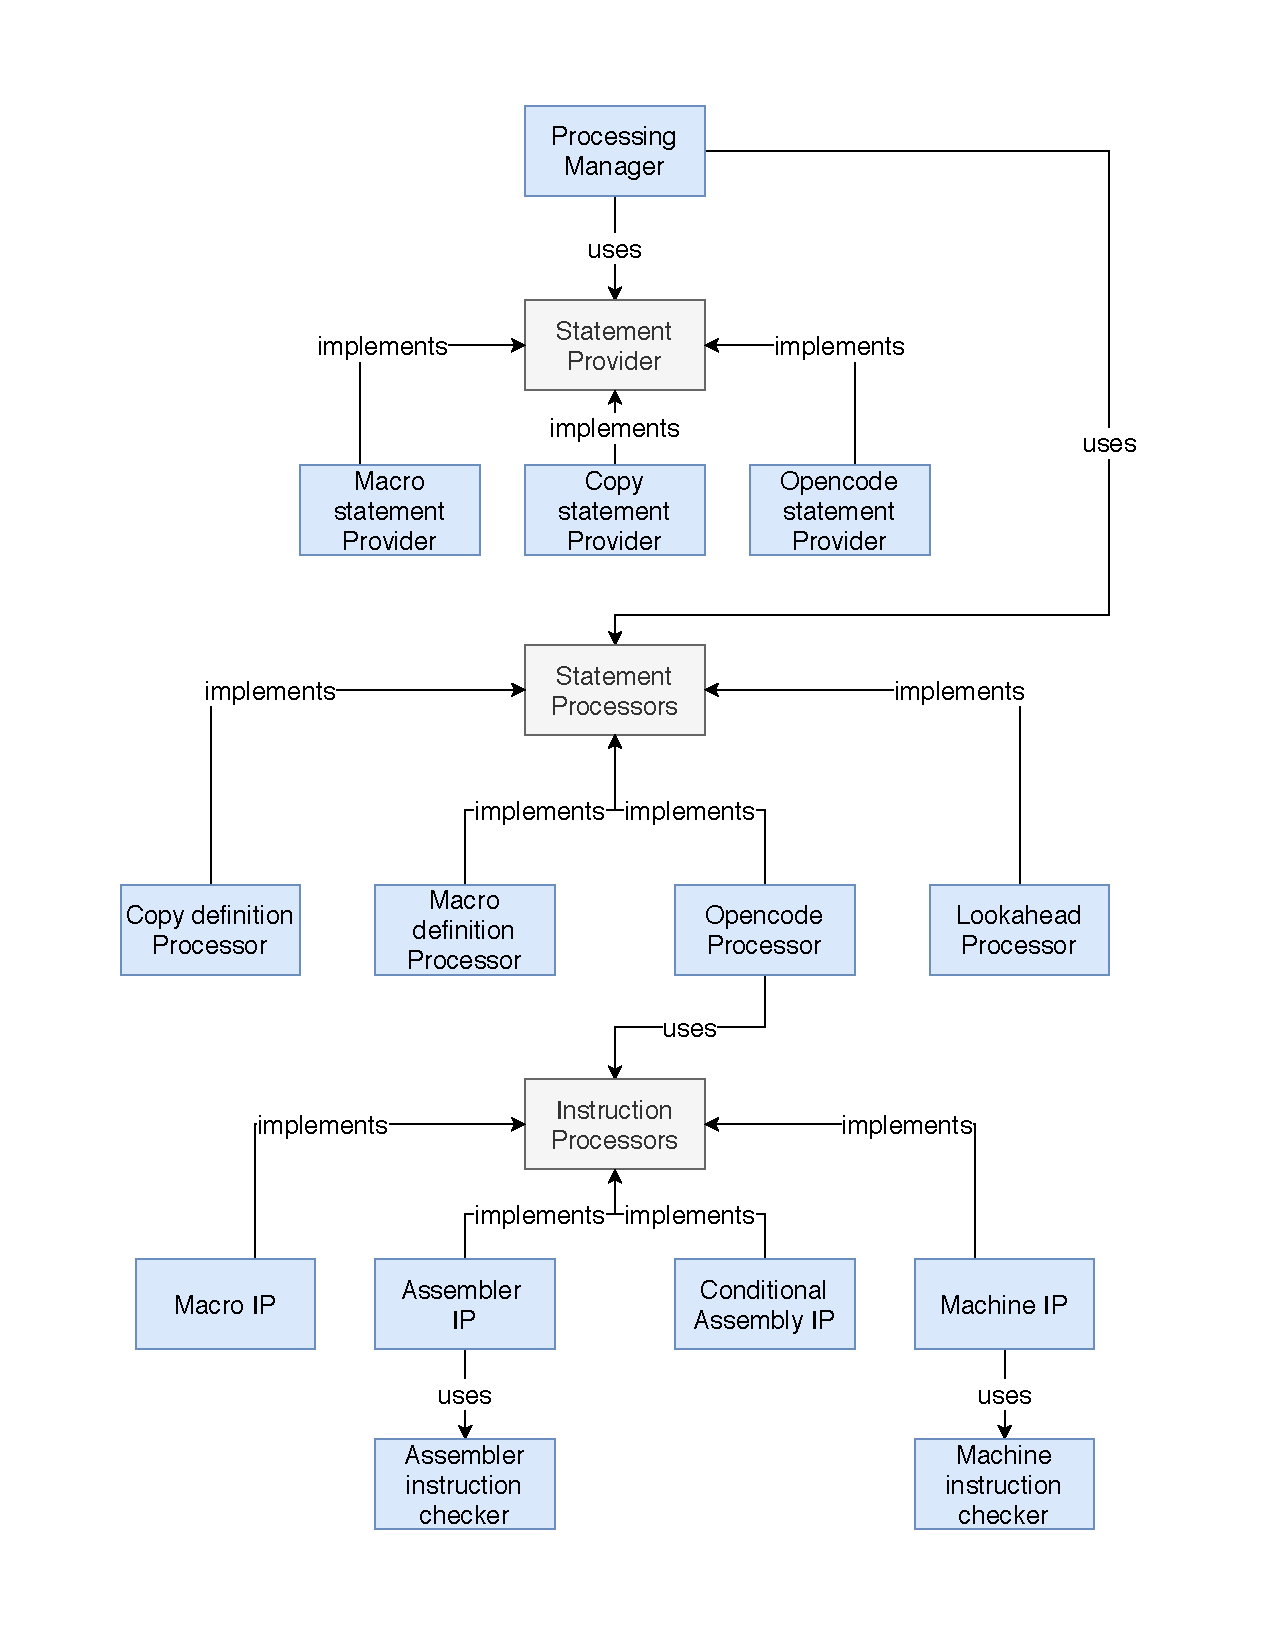
\includegraphics[width=\textwidth]{img/processing_manager_arch}
	\caption{The architecture of Processing manager}
	\label{fig06:proc_mngr}
\end{figure}

\subsection{Overview}

To construct processing manager, analyzer passes this objects to the constructor:
\begin{itemize}
	\item \emph{Parser} that provide statements from the processed file. Further on in this chapter, we will refer to the parser as to the \emph{Opencode statement provider}.
	\item \emph{HLASM context tables} that hold current state of the parsed source.
	\item \emph{Library data} defining the initial state of the manager.
	\item \emph{Name} of the processed file.
	\item \emph{Parse library provider} to solve in file dependencies.
	\item \emph{Statement fields parser} for parsing deferred statements. 
\end{itemize}

As the processing of the HLASM source file is rather complicated, we defined a \emph{statement provider} for each different source of statements and a \emph{statement processor} for each different manner of statement processing. Therefore, processing manager contains two arrays, each consisting of different instance of statement processor, or statement provider.  Also, it has notion of the processor or provider that is in the current use and implement interfaces that change them.

\subsection{The main loop}

The main loop of the processing works with the current processor and provider. In the loop body --- as the names suggest --- statement provider provides next statement for statement processor that processes it accordingly. The loop breaks when the last processor finishes work.

When provider or processor finishes its work, it is replaced with another. The following rules apply:

\begin{enumerate}
	\item When a processor finishes it's work, the next processor is selected from the array.
	\item When a provider finishes --- before the next provider is selected from the array --- manager checks whether the provider's end triggers finishing of the current processor as well (next referred as \emph{terminal condition}). If true, performs rule 1.
\end{enumerate}

\subsection{Statement}

Statement consists of \emph{statement fields} --- \emph{label field}, \emph{instruction field}, \emph{operands field}, \emph{remark field}. It is used by statement processors and produced by statement providers. 

The abstract class \emph{HLASM statement} is the ancestor for all statement related classes. Then, abstract classes \emph{deferred} and \emph{resolved} statements follow. Deferred statement states that operand field is stored in string format as the concrete format is yet not known. Resolved statements are complementary to the deferred statements. Concrete implementation of this statements are used throughout the processing.

\subsection{Statement Processors}
\label{lab06:sect_proc}

The motivation in distinguishing different statement processors was the complexity of the HLASM language. There are many cases when the same statements require different processing under different circumstances (e.g. COPY instruction in macro is handled differently than in opencode, or lookahead mode can accept statements that would fail to be processed by ordinary processing).

In processing manager's array, statement processors can not be assigned a priority nor can be statically organized in an array. Rather they are dynamically assigned to the manager's array when needed and removed from the array when they finish.


\subsubsection{Copy and Macro definition Processors}

Both of this statement processors handle statement collecting, forming definition structure and storing it into HLASM context tables. They come into effect when COPY instruction is encountered in the source code or macro definition respectively. 

The statements collected into the copy or macro definition are mainly deferred statements. That is because HLASM nature allows instruction aliasing. Therefore, in the definition processing, as an instruction field is parsed, we still do not know a format of the operands. The format is fully deduced when the definition is handled to a provider and processed by opencode processor.

However, some statements in the macro and copy definition forbid aliasing and the operand format can be deduced (e.g. conditional assembly instructions in macro definition). This leads to the processor's necessity to ask provider to retrieve statement with correct format according to the deduced format based on the provided instruction  (see \cref{lab06:proc_stat}).

\subsubsection{Lookahead Processors}

Lookahead processor is activated when currently processed conditional assembly statement require value of the ordinary or sequence symbol that is not previously defined. It looks through following statements and finishes when the target symbol is found or when all the statement providers are exhausted.

\subsubsection{Opencode Processors}

Opencode processor's (in code described as Ordinary processor) usage can be described in the following points:
\begin{enumerate}
	\item If model statement is encountered (see \cref{var_sym}), it substitutes the variable symbols and resolves the statement.
	\item Checks statement for validity.
	\item Performs instruction in the manner of updating HLASM context tables with help of \emph{instruction processors}.
\end{enumerate}

\vspace{0.5cm}

During their work, any processor can encounter statement that require processor change (e.g. encountering special instruction or non previously defined sequence symbol, see \cref{tab06:processor_change}). Therefore, they use interface \emph{processing state listener} (implemented by processing manager) that tells manager to change the current processor.

If we look at the \cref{tab06:processor_change}, we can see that it does not have field that starts Opencode processor. This is because the processor is set as a default by the manager. The next think we can see is that Copy processor does not finish itself during it's work. That is because it  can be finished only by it's terminal condition (see \cref{tab06:term_cond}). 

\begin{table}
	\centering
	\begin{tabular}{lccccc}
		                   & \thead{\textbf{END}\\ \textbf{instruction}} & \thead{\textbf{COPY}\\ \textbf{instruction}} & \thead{\textbf{MACRO}\\ \textbf{instruction}} & \thead{\textbf{MEND}\\ \textbf{instruction}} & \thead{\textbf{undefined} \\ \textbf{symbol}} \\ \toprule
		\textbf{Opencode}  &                 finish self                 &                 starts Copy                  &                 starts Macro                  &                                              &               starts Lookahead                \\
		\textbf{Copy}      &                                             &                                              &                                               &                                              &                                               \\
		\textbf{Macro}     &                                             &                 starts Copy                  &                                               &                 finish self                  &                                               \\
		\textbf{Lookahead} &                 finish self                 &                 starts Copy                  &                                               &                                              &                                               \\ \bottomrule
	\end{tabular}
	\caption{Description of statement processor changes.}
	\label{tab06:processor_change}
\end{table}

\subsection{Statement Providers}

In contrary to statement processors, statement providers are stored in the array based on the priority (lower index, greater priority):

\begin{enumerate}
	\item Macro definition statement provider
	\item Copy definition statement provider
	\item Opencode statement provider
\end{enumerate}

Based on the priority, each cycle of the processor's main loop, providers are checked whether it has statements to provide. That is because after each cycle, a processor with greater priority than the current one can be activated. 

\begin{table}
	\centering
	\begin{tabular}{lccc}
		                   & \thead{\textbf{Macro provider} \\ \textbf{ends}} & \thead{\textbf{Copy provider} \\ \textbf{ends}} & \thead{\textbf{Opencode provider} \\ \textbf{ends}} \\ \toprule
		\textbf{Opencode}  &                                                  &                                                 &                     finish self                     \\
		\textbf{Copy}      &                                                  &                                                 &                     finish self                     \\
		\textbf{Macro}     &                   finish self                    &                                                 &                     finish self                     \\
		\textbf{Lookahead} &                   finish self                    &                                                 &                     finish self                     \\ \bottomrule
	\end{tabular}
	\caption{Description of statement processors' terminal condition.}
	\label{tab06:term_cond}
\end{table}

For the main loop to be correctly defined, opencode provider's finish triggers terminal condition for all statement processors. Hence, when opencode provider finishes then all the processors finish as well and processing ends (see \cref{tab06:term_cond}).

\subsubsection{Statement passing}
\label{lab06:proc_stat}

In HLASM language, it is difficult to parse statements into one common structure due to major differences in operand field of different instruction formats. Moreover, when parsing statements, the instruction format is not yet known due to aliasing. Therefore, operand fields are stored as strings. This option, however, puts responsibility to produce correct statement format during statement passing when instruction format is deduced. The following rules apply (also see \cref{fig06:process_next}):

\begin{enumerate}
	\item Provider retrieves the instruction field part of the statement.
	\item Provider calls processor's \texttt{get\_processing\_status} method with instruction field as a parameter.
	\item Return value of the call determines the required format of the operand field for the processor.
	\item With the return value, provider passes correct statement format to the processor. 
\end{enumerate}

\begin{figure}
	\centering
	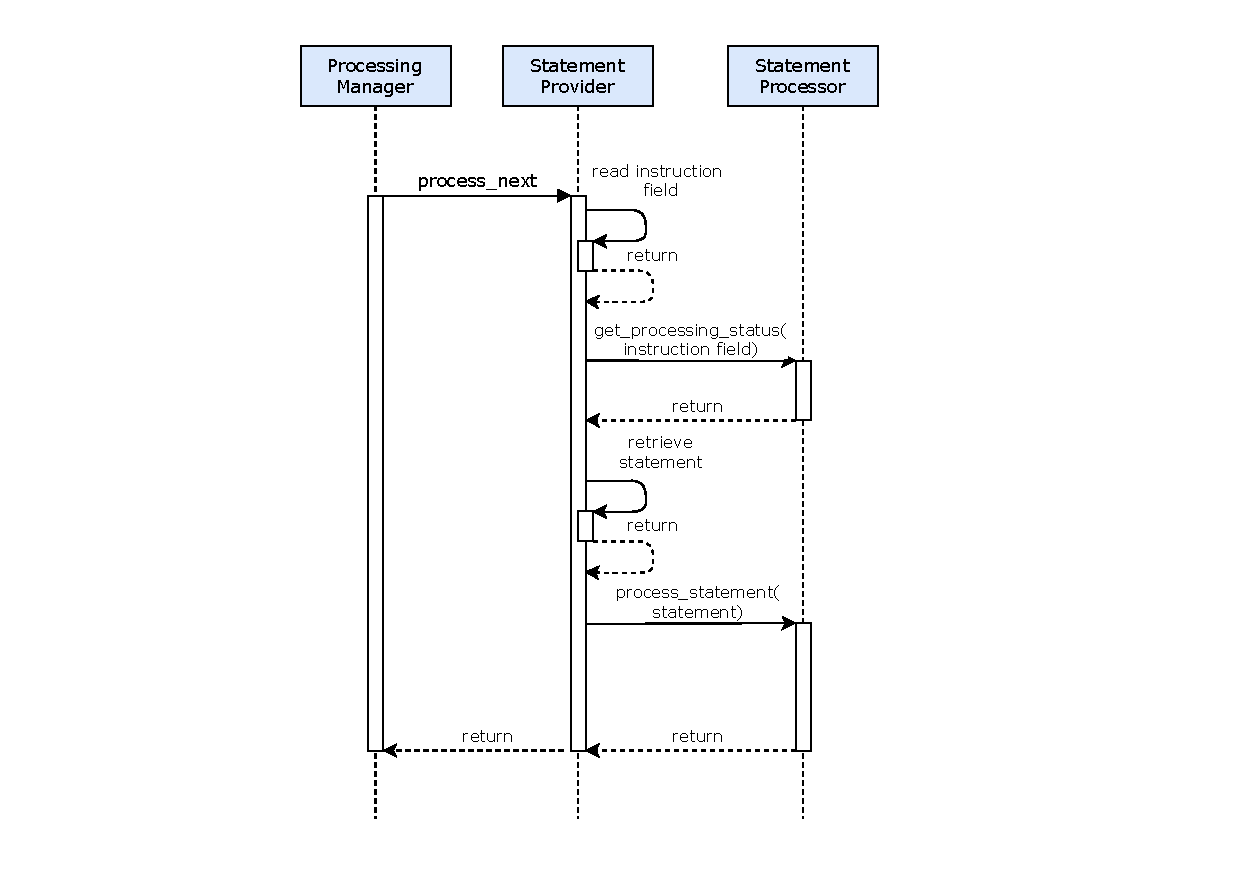
\includegraphics[width=13cm]{img/process_next}
	\caption{The process of statement passing.}
	\label{fig06:process_next}
\end{figure}


\subsubsection{Copy and Macro definition Provider}

This providers are activated  when COPY instruction copies a file into the source code or when a macro is visited respectively. They provide a sequence of statements to an arbitrary processor until all statements from the copy or macro definition are provided. Then, if there is no nested invocation, provider with lower priority is selected.

\subsubsection{Opencode Provider}

Opencode provider is active as long as there are statements in the source file. It retrieves statements from the source code with help of lexer and parser (see \cref{lab06:parser}).

\subsection{Manager's initial state}
\label{lab06:lib_data}
Having described processors and providers, we are ready to talk about which of them are initialized by the manager at the beginning of the processing. The manager determines this by library data passed by analyzer.

Library data contains a file name and enumeration telling the meaning of the file that is being parsed --- \emph{processing kind}.

\emph{Ordinary} processing kind states that the file being processed is the main source file (in HLASM jargon called open-code). It is the beginning processing file. With this information, manager initializes all the statement providers with respective order and \emph{only} opencode processor. This enumeration is passes when analyzer has owner semantics.

\emph{Copy} and \emph{Macro} processing kinds describe that manager will process source code that contains copy or macro definition respectively. Hence, \emph{only} copy  definition processor or macro definition processor is initialized. Also, all but macro statement provider are initialized. That is because macro definitions would pollute statement sources (i.e. when parse library provider is called within macro call). Also, no macros will be visited nor needed as a statement source when processing a new source code. This enumeration is passes when analyzer has reference semantics.


\subsection{Statement field parser}
\label{lab06:field_parser}

Statement field parser is an interface passed to the statement providers by processing manager implemented by the parser (see \cref{lab06:parser}).

Firstly, it is used during statement passing. In some cases provider is requested a concrete format of a string-stored statement. The string is re-parsed with the according format. Then the field is returned back to the statement provider. 

Another use of field parser is in opencode processor as model statements are resolved there. After variable symbol substitution, the resulting string field is re-parsed with field parser.

\subsection{Instruction processors}

Used by ordinary processor, instruction processors are helper classes that divide processing of HLASM instruction types.

There are four specialized instruction processors:
\paragraph*{Macro IP} looks up for macro definition in HLASM context tables and calls it.
\paragraph*{Assembler and Machine IP} process assembler and machine instructions (see \cref{asm_instrs} \cref{mach_instr}) to retain consistency in HLASM context tables.

\paragraph*{Conditional assembly IP} executes conditional assembly instructions (see \cref{ca_instr}). 

\vspace{5mm}

See the current list of processed instruction in \cref{tab06:instr_proc}.

\begin{table}
	\centering
	\begin{tabular}{lr}
		\textbf{IP}                   &                  \textbf{Processed instructions} \\ \toprule
		\textbf{Assembler}            & *SECT, COM, LOCTR, EQU, DC, DS, COPY, EXTRN, ORG \\
		\textbf{Machine}              &                                      \emph{NONE} \\
		\textbf{Macro}                &                                       \emph{ANY} \\
		\textbf{Conditional Assembly} &    SET*, GBL*, ANOP, ACTR, AGO, AIF, MACRO, MEND \\ \bottomrule
	\end{tabular}
	\caption{Table of instructions that are processed by instruction processors.}
	\label{tab06:instr_proc}
\end{table}

\subsubsection{Expressions}

distinguished into CA and ASM expressions. 
image with arch
overview

they are parsed in grammar, later you give an expression "symbol evaluator" and it returns its value




\subsubsection{Data definition}

validation and processing purpose